\subsection{Stabilit"at linearer Systeme}
Die Stabilit"at linearer Systeme $\diffp{}{t}x(t) = A \cdot x(t)$ mit regul"arer $2 \times 2$-Matix $A$\\

\begin{tabular}{|l|l|l|}
	\hline
	\textbf{Eigenwerte}                                  & \textbf{Klassifizierung}                & \textbf{Stabilit"at} \\ \hline
	$\lambda_1 > \lambda_2 > 0$                          & Knoten                                  & instabil             \\ \hline
	$\lambda_1 < \lambda_2 < 0$                          & Knoten                                  & asymptotisch stabil  \\ \hline
	$\lambda_2 <  0 < \lambda_1 $                        & Sattelpunkt                             & instabil             \\ \hline
	$\lambda_1 = \lambda_2  > 0$                         & eigentlicher oder uneigentlicher Knoten & instabil             \\ \hline
	$\lambda_1 = \lambda_2 < 0$                          & eigentlicher oder uneigentlicher Knoten & asymptotisch stabil  \\ \hline
	$\lambda_1 , \lambda_2 = \mu \pm i \cdot \nu$ mit    & Spiralpunkt                             &  \\
	$\mu > 0$                                            &                                         & instabil             \\
	$\mu < 0$                                            &                                         & asymptotisch stabil  \\ \hline
	$\lambda_1 = i\cdot \nu ,  \lambda_2 = -i \cdot \nu$ & Zentrum                                 & stabil               \\ \hline
\end{tabular} 

\subsection{Stabilit"at linearer Systeme mit reellen Koeffizienten}
\begin{subequations}
	\begin{equation*}
		\lambda^2 + p \lambda + q = 0
	\end{equation*}
	\begin{equation*}
		\lambda_{1,2} = \frac{1}{2} \cdot (p \pm \sqrt{\Delta}) \quad \text{mit} \quad \Delta = p^2 -4q
	\end{equation*}
\end{subequations}\\ \\

\begin{minipage}[h]{0.35\textwidth} 
	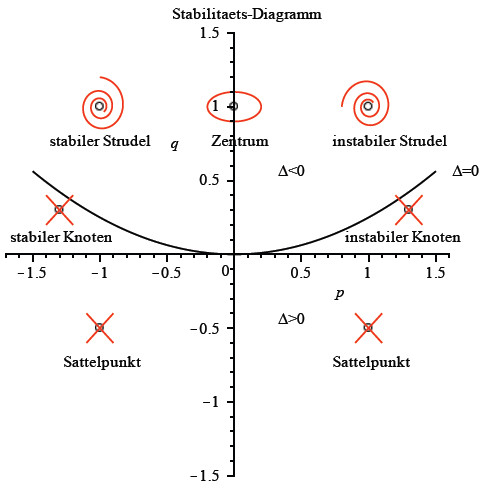
\includegraphics[width=0.9\textwidth]{images/StabilitaetsDiagramm.png}
\end{minipage}
\begin{minipage}[h]{0.35\textwidth}
	F"ur $\Delta > 0$ gilt:\\
	\begin{tabular}{|l|l|l|}
		\hline
		\textbf{Parameter $p$ und $q$} & \textbf{Eigenwerte}               & \textbf{Stabilit"at} \\ \hline
		$p,q > 0$                      & $\lambda_1 >0$ und $\lambda_2 >0$ & instabiler Knoten                        \\ \hline
		$p>0 ,  q<0$                   & $\lambda_1 >0$ und $\lambda_2 <0$ & Sattelpunkt                              \\ \hline
		$p< 0, q>0$                    & $\lambda_1 <0$ und $\lambda_2 >0$ & stabiler Knoten                          \\ \hline
		$p<0, q<0$                     & $\lambda_1 <0$ und $\lambda_2 >0$ & Sattelpunkt                              \\ \hline
	\end{tabular} \\ \\
	
	F"ur $\Delta = 0$ gilt:\\
	\begin{tabular}{|l|l|l|}
		\hline
		\textbf{Parameter $p$} & \textbf{Eigenwerte}        & \textbf{Stabilit"at}                         \\ \hline
		$p> 0$                         & $\lambda_1 = \lambda_2 >0$ & instabiler eigen-/ uneigentlicher Knoten \\ \hline
		$p< 0$                         & $\lambda_1 = \lambda_2 <0$ & stabiler eigen- / uneigentlicher Knoten   \\ \hline
	\end{tabular}\\ \\
	
	F"ur $\Delta < 0$ gilt:\\
		\begin{tabular}{|l|l|l|}
			\hline
			\textbf{Parameter $p$} & \textbf{Eigenwerte}                           & \textbf{Stabilit"at} \\ \hline
			$p> 0$                         & $\lambda_1 , \lambda_2 = \mu \pm i \cdot \nu$ & instabilen Strudel   \\ \hline
			$p< 0$                         & $\lambda_1 , \lambda_2 = \mu \pm i \cdot \nu$ & stabilen Strudel     \\ \hline
			$p= 0$                         & $\lambda_1 = \lambda_2 <0$                    & Zentrum              \\ \hline
		\end{tabular}  
\end{minipage}


